\documentclass[12pt]{article}
\usepackage[english]{babel}
\usepackage[utf8]{inputenc}

%% Pointer to 'default' preamble, other reusable files
% pacakages and definitions

\usepackage{geometry}
\geometry{
	letterpaper, 
	portrait, 
	top=.75in,
	left=.8in,
	right=.75in,
	bottom=.5in		} 	% Page Margins
	
%% additional packages for nice things
\usepackage{amsmath} 	% for most math
\usepackage{commath} 	% for abs
\usepackage{lastpage}	% for page count
\usepackage{amssymb} 	% for therefore
\usepackage{graphicx} 	% for image handling
\usepackage{wrapfig} 	% wrap figures
\usepackage[none]{hyphenat} % for no hyphenations
\usepackage{array} 		% for >{} column characterisctis
\usepackage{physics} 	% for easier derivative \dv....
\usepackage{tikz} 		% for graphic@!
\usepackage{circuitikz} % for circuits!
\usetikzlibrary{arrows.meta} % for loads
\usepackage[thicklines]{cancel}	% for cancels
\usepackage{xcolor}		% for color cancels
\usepackage[per-mode=fraction]{siunitx} % for si units and num
\sisetup{group-separator = {,}, group-minimum-digits = 3} % additional si unit table functionality

\usepackage{fancyhdr} 	% for header
\usepackage{comment}	% for ability to comment out large sections
\usepackage{multicol}	% for multiple columns using multicols
\usepackage[framed,numbered]{matlab-prettifier} % matlab sytle listing
\usepackage{marvosym} 	% for boltsymbol lightning
\usepackage{pdflscape} 	% for various landscape pages in portrait docs.
%\usepackage{float}
\usepackage{fancyvrb}	% for Verbatim (a tab respecting verbatim)
\usepackage{enumitem}	% for [resume] functionality of enumerate
\usepackage{spreadtab} 	% for using formulas in tables}
\usepackage{numprint}	% for number format in spread tab
\usepackage{subcaption} % for subfigures with captions
\usepackage[normalem]{ulem} % for strike through sout

% for row colors in tables....
\usepackage{color, colortbl}
\definecolor{G1}{gray}{0.9}
\definecolor{G2}{rgb}{1,0.88,1}%{gray}{0.6}
\definecolor{G3}{rgb}{0.88,1,1}

% For table formatting
\usepackage{booktabs}
\renewcommand{\arraystretch}{1.2}
\usepackage{floatrow}
\floatsetup[table]{capposition=top} % put table captions on top of tables

% Caption formating footnotesize ~ 10 pt in a 12 pt document
\usepackage[font={small}]{caption}

%% package config 
\sisetup{output-exponent-marker=\ensuremath{\mathrm{E}}} % for engineer E
\renewcommand{\CancelColor}{\color{red}}	% for color cancels
\lstset{aboveskip=2pt,belowskip=2pt} % for more compact table
%\arraycolsep=1.4pt\def
\setlength{\parindent}{0cm} % Remove indentation from paragraphs
\setlength{\columnsep}{0.5cm}
\lstset{
	style      = Matlab-editor,
	basicstyle = \ttfamily\footnotesize, % if you want to use Courier - not really used?
}
\renewcommand*{\pd}[3][]{\ensuremath{\dfrac{\partial^{#1} #2}{\partial #3}}} % for larger pd fracs
\renewcommand{\real}[1]{\mathbb{R}\left\{ #1 \right\}}	% for REAL symbol
\newcommand{\imag}[1]{\mathbb{I}\left\{ #1 \right\}}	% for IMAG symbol
\definecolor{m}{rgb}{1,0,1}	% for MATLAB matching magenta
	
%% custom macros
\newcommand\numberthis{\addtocounter{equation}{1}\tag{\theequation}} % for simple \numberthis command

\newcommand{\equal}{=} % so circuitikz can have an = in the labels
\newcolumntype{L}[1]{>{\raggedright\let\newline\\\arraybackslash\hspace{0pt}}m{#1}}
\newcolumntype{C}[1]{>{\centering\let\newline\\\arraybackslash\hspace{0pt}}m{#1}}
\newcolumntype{R}[1]{>{\raggedleft\let\newline\\\arraybackslash\hspace{0pt}}m{#1}}

%% Header
\pagestyle{fancy} % for header stuffs
\fancyhf{}
% spacing
\headheight 29 pt
\headsep 6 pt
%%% custom commands for nicer units
\newcommand{\mw}{\ensuremath{\text{ MW}}}
\newcommand{\hz}{\ensuremath{\text{ Hz}}}
\newcommand{\pu}{\ensuremath{\text{ Pu}}}
\newcommand{\sbase}{\ensuremath{\text{S}_{\text{Base}}}}
\newcommand{\fbase}{\ensuremath{f_{\text{Base}}}}
\newcommand{\mbase}[1]{\ensuremath{\text{M}_{\text{Base}_{#1}}}}
\newcommand{\hsys}{\ensuremath{\text{ H}_{\text{sys}}}}


%% Header
\rhead{Thad Haines \\ Page \thepage\ of \pageref{LastPage}}
\chead{Collection of BA Descriptions and Options \\  }
\lhead{Research \\ October 14th, 2019 }

% For figure usage and linking
\usepackage{graphicx}

% Easy template for testing table builds to verify their appearance.
%\documentclass[]{report} 
%\usepackage{geometry}
%\geometry{letterpaper, margin=1in}
\usepackage{pdflscape}
\usepackage{booktabs} 	% enhanced table qualities

\usepackage[per-mode=fraction]{siunitx} % for si units and num

\usepackage{array} 		% for >{} column characterisctis
\newcolumntype{L}[1]{>{\raggedright\let\newline\\\arraybackslash\hspace{0pt}}m{#1}}
\newcolumntype{C}[1]{>{\centering\let\newline\\\arraybackslash\hspace{0pt}}m{#1}}
\newcolumntype{R}[1]{>{\raggedleft\let\newline\\\arraybackslash\hspace{0pt}}m{#1}}
%\pagestyle{empty}

\begin{document}


%\pagebreak
\begin{figure}[!ht]
	\centering
	\footnotesize
	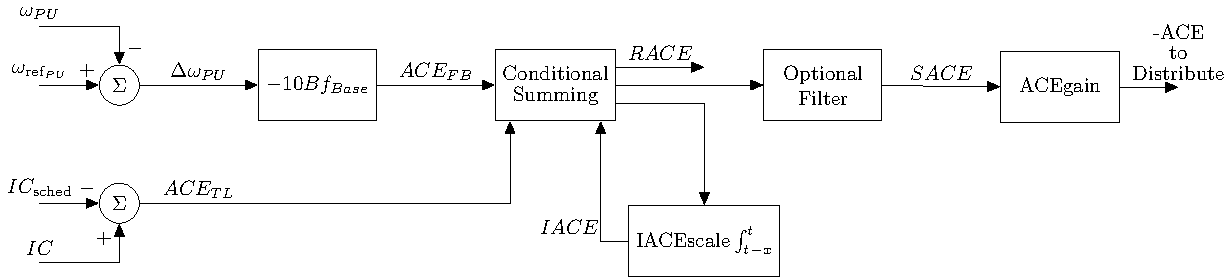
\includegraphics[width=\linewidth]{../../models/AGC-TLB/AGC-TLB}
	\caption{Block diagram of ACE calculation and manipulation.}
	\label{fig: AGC-TLB}
\end{figure}\vspace{-1em} % will remove 1 white space after image - typically good

\begin{figure}[!ht]
	\centering
	\footnotesize
	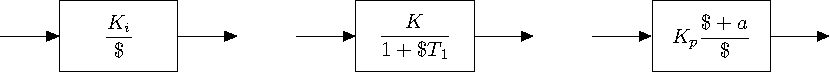
\includegraphics[width=.8\linewidth]{../../models/filterAgents/filterAgent}
	\caption{Block diagram available filters.}
	\label{fig: filterAgents}
\end{figure}\vspace{-1em} % will remove 1 white space after image - typically good


\input{../../tables/TLBoptions/TLBoptions}

If IACE is to be added using the weight option:
\[ACE = ACE*(1-IACEweight)+ IACE*IACEweight*IACEscale\]
Else:
\[ACE = ACE+IACE*IACEscale\]


\begin{figure}[!ht]
	\centering
	\footnotesize
	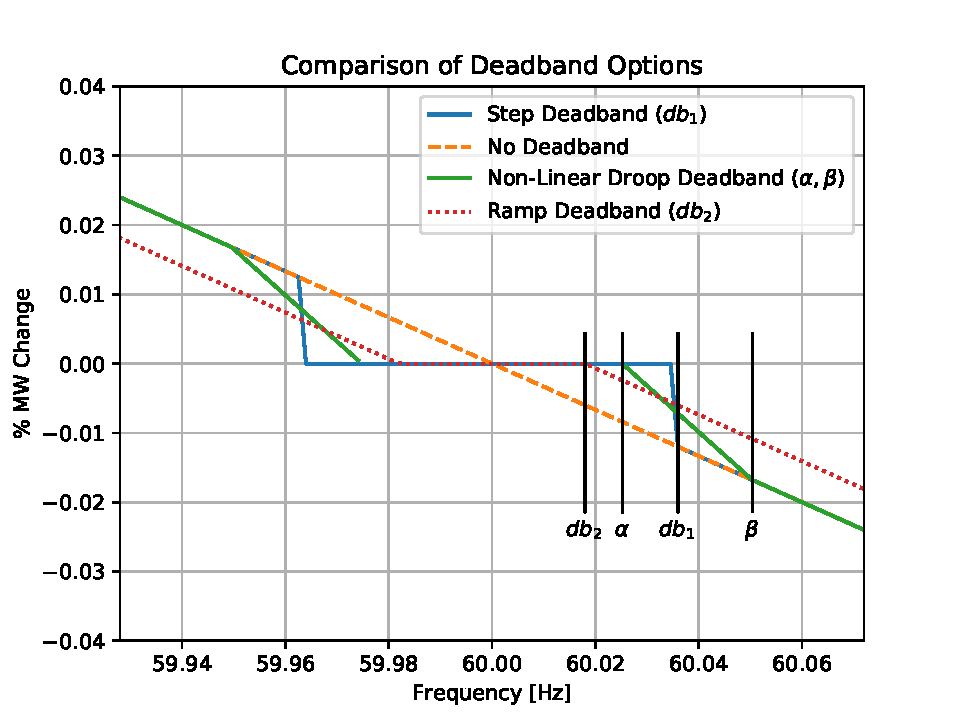
\includegraphics[width=.5\linewidth]{dbAction}
	\caption{Governor deadband options.}
	\label{fig: dbAction}
\end{figure}\vspace{-1em} % will remove 1 white space after image - typically good


\pagebreak
% File for BAdict
% NOTE: the body of this table was made in EXCEL, though has been updated in this file further than in excel due to latex formating etc.
\begin{landscape}
\begin{table}[!ht]
	\centering
	\begin{tabular}{@{} llllp{4in} @{}} 	
		\toprule % @ signs to remove extra L R space
		\footnotesize % this will affect the table font (makse it 10pt)
		\raggedright % for non justified table text
		Key	&	Type	&	Units	&	Example	&	Description	\\	
		\midrule		
		B	&	String	&	MW/0.1Hz	&	"1.0 : permax"	&	Describes the frequency bias scaling factor B used in the ACE calculation. Various Options exist.	\\
		AGCActionTime	&	Float	&	Seconds	&	5	&	Time between AGC dispatch messages.	\\
		AGCType	&	String	&	-	&	"TLB : 2"	&	Dictates which AGC routine to use and type specific options.	\\
		UseAreaDroop	&	Boolean	&	-	&	False	&	If True, all governed generators under BA control will use the area droop.	\\
		AreaDroop	&	Float	&	Hz/MW	&	0.05	&	Droop value to use if 'UseAreaDroop' is True.	\\
		IncludeIACE	&	Boolean	&	-	&	True	&	If True, include IACE in ACE calculation	\\
		IACEconditional	&	Boolean	&	-	&	False	&	Adds IACE to ACE if signs of deltaw, ACE and IACe all match.	\\
		IACEwindow	&	Integer	&	Seconds	&	60	&	Defines the length of moving integration window to use in IACE. If set to 0, integration takes place for all time.	\\
		IACEscale	&	Float	&	-	&	0.0167	&	Value used to scale IACE.	\\
		IACEweight	&	Float	&	-	&	0.5	&	Weighting of IACE to ACE used during summation.	\\
		IACEdeadband	&	Float	&	Hz	&	0.036	&	Absolute value of system frequency where IACE will not be calculated below.	\\
		ACEFiltering	&	String	&	-	&	'PI : 0.03 0.001'	&	String used to dictate which filter agent is created and specific parameters.	\\
		AGCDeadband	&	Float	&	MW	&	1.5	&	Value of ACE to ignore sending in AGC dispatch. Not implemented as of this writing.	\\
		GovDeadbandType	&	String	&	-	&	step'	&	Type of deadband to be applied to area governors.	\\
		GovDeadband	&	Float	&	Hz	&	0.036	&	Absolute value of system frequency that governors will not respond below.	\\
		GovAlpha	&	Float	&	Hz	&	0.016	&	Specific to 'NLDroop' type of deadband. Specifies lower bound of non-linear droop.	\\
		GovBeta	&	Float	&	Hz	&	0.036	&	Specific to 'NLDroop' type of deadband. Specifies upper  bound of non-linear droop and return to specified machine droop.	\\
		CtrlGens	&	List of Strings	&	-	&	-	&	List of generators, participation factor, and dispatch signal type.	\\
		\bottomrule
	\end{tabular}
	\caption{Balancing Authority dictionary input information.}
	\label{tab:BADict}
\end{table}
\end{landscape} % landscape

\end{document}